\documentclass[11pt]{article}

%  USE PACKAGES  ---------------------- 
\usepackage[margin=0.7in,vmargin=1in]{geometry}
\usepackage{amsmath,amsthm,amsfonts}
\usepackage{amssymb}
\usepackage{fancyhdr}
\usepackage{enumerate}
\usepackage{mathtools}
\usepackage{hyperref,color}
\usepackage{enumitem,amssymb}
\newlist{todolist}{itemize}{4}
\setlist[todolist]{label=$\square$}
\usepackage{pifont}
\newcommand{\cmark}{\ding{51}}%
\newcommand{\xmark}{\ding{55}}%
\newcommand{\done}{\rlap{$\square$}{\raisebox{2pt}{\large\hspace{1pt}\cmark}}%
\hspace{-2.5pt}}
\newcommand{\HREF}[2]{\href{#1}{#2}}
\usepackage{textcomp}
\usepackage{listings}
\usepackage{array}
\lstset{
basicstyle=\small\ttfamily,
% columns=flexible,
upquote=true,
breaklines=true,
showstringspaces=false
}
%  -------------------------------------------- 

%  HEADER AND FOOTER (DO NOT EDIT) ----------------------
\newcommand{\problemnumber}{0}
\pagestyle{fancy}
\fancyhead{}
\fancyhead[L]{\textbf{Question \problemnumber}}
\newcommand{\newquestion}[1]{
\clearpage % page break and flush floats
\renewcommand{\problemnumber}{#1} % set problem number for header
\phantom{}  % Put something on the page so it shows
}
\fancyfoot[L]{IE 332}
\fancyfoot[C]{Assignment submission}
\fancyfoot[R]{Page \thepage}
\renewcommand{\footrulewidth}{0.4pt}

%  --------------------------------------------


%  COVER SHEET (FILL IN THE TABLE AS INSTRUCTED IN THE ASSIGNMENT) ----------------------
\newcommand{\addcoversheet}{
\clearpage
\thispagestyle{empty}
\vspace*{0.5in}

\begin{center}
\Huge{{\bf IE332 Project \#2}} % <-- replace with correct assignment #

Due: April 28th, 11:59pm EST % <-- replace with correct due date and time
\end{center}

\vspace{0.3in}

\noindent We have {\bf read and understood the assignment instructions}. We certify that the submitted work does not violate any academic misconduct rules, and that it is solely our own work. By listing our names below we acknowledge that any misconduct will result in appropriate consequences. 

\vspace{0.2in}

\noindent {\em ``As a Boilermaker pursuing academic excellence, I pledge to be honest and true in all that I do.
Accountable together -- we are Purdue.''}

\vspace{0.3in}

\begin{table}[h!]
  \begin{center}
    \label{tab:table1}
    \begin{tabular}{c| m{5em} m{5em} m{5em} m{5em} m{3em} |c|c}
      Student & Algorithm Development & Complexity Analysis & Implemen-tation & Performance Analysis/Testing & Report & Overall & DIFF\\
      \hline
      Annie Zhang & 10 & 60 & 10 & 10 & 10 & 100 & 0\\
      Caroline Cudney & 10 & 10 & 60 & 10 & 60 & 100 & 0\\
      Hrishabh Nadkarni & 60 & 10 & 10 & 10 & 10 & 100 & 0\\
      Mounzr Nabulsi & 10 & 10 & 10 & 10 & 10 & 50 & 50\\
      Yuze Tang & 10 & 10 & 10 & 60 & 10 & 70 & 30\\
      \hline
      St Dev & 20 & 20 & 20 & 20 & 20 & 44.27 & 44.27
    \end{tabular}
  \end{center}
\end{table}

\vspace{0.2in}

\noindent Date: \today.
}
%  -----------------------------------------

%  TODO LIST (COMPLETE THE FULL CHECKLIST - USE AS EXAMPLE THE FIRST CHECKED BOXES!) ----------------------
\newcommand{\addtodo}{
\clearpage
\thispagestyle{empty}

\section*{Read Carefully. Important!}

\noindent By electronically uploading this assignment to Brightspace you acknowledge these statements and accept any repercussions if in any violation of ANY Purdue Academic Misconduct policies. You must upload your homework on time for it to be graded. No late assignments will be accepted. {\bf Only the last uploaded version of your assignment before the due date will be graded}.

\vspace{0.2in}

\noindent {\bf NOTE:} You should aim to submit no later than 30 minutes before the deadline, as there could be last minute network traffic that would cause your assignment to be late, resulting in a grade of zero. 

\vspace{0.2in}

\noindent When submitting your assignment it is assumed that every student considers the below checklist, as there are grading consequences otherwise (e.g., not submitting a cover sheet is an automatic grade of ZERO).

\begin{todolist}

    \item[\done] Your solutions were prepared using the \LaTeX template provided in Brightspace. 
    \item[\done] Your submission has a cover sheet as its first page and this checklist as its second page, according to the template provided.
	 \item All of your solutions (program code, etc.) are included in the submission as requested. % Check this checkbox and the following ones if satisfied <---
    \item You have not included any screen shots, photos, etc. (plots should be intermediately saved as .png files and then added into your .tex file). % <---
	 \item All math notation and algorithms (algorithmic environment) are created using appropriate \LaTeX code (no pictures, handwritten solutions, etc.). % <---
    \item The .pdf is submitted as an individual file and not in a {\tt .zip}.
    \item You kept the \LaTeX source code in your files until this assignment is graded, in case you are required to show proof of creating your assignment using \LaTeX.  % <---
    \item If submitting with a partner, your partner is added in the submission section in Gradescope after you upload your file. % <---
    \item You have correctly matched each question to its page \# in the .pdf submission in the Gradescope section (after you uploaded your file).
    \item Watch videos on creating pseudocode if you need a refresher or quick reference to the idea. These are good starter videos:    % <---
    
     \HREF{https://www.youtube.com/watch?v=4jLO0vXPktU}{www.youtube.com/watch?v=4jLO0vXPktU} 
    
    \HREF{https://www.youtube.com/watch?v=yGvfltxHKUU}{www.youtube.com/watch?v=yGvfltxHKUU}
\end{todolist}
}

%% LaTeX
% Für alle, die die Schönheit von Wissenschaft anderen zeigen wollen
% For anyone who wants to show the beauty of science to others

%  -----------------------------------------


\begin{document}


\addcoversheet
\addtodo

% BEGIN YOUR ASSIGNMENT HERE:
\newquestion{Table of Contents}

%TABLE OF CONTENTS
\tableofcontents

%MAIN TEXT OF REPORT
\pagebreak
\newquestion{Report}
\section{Introduction}
\addcontentsline{toc}{section}{Project}
\section*{Project}
Binary classifiers are a type of supervised machine learning algorithms that are used to split objects into one of two groups or classes. They are often used in medical evaluations when diagnosing a patient as positive or negative and have other applications including email spam and quality assurance. The binary classifier for this project focuses on identifying whether images were showing dandelions or just grass by computing a percentage. The code outputs two separate percents per image. The first percent is the amount it predicts that the image is a dandelion, and the second percent is the amount the algorithm predicts the image is of grass. If it is over 50 for the first percent, then the algorithm declares that the image is of dandelions, otherwise it says it is grass because the second percent would then be over 50. The goal of the project is to implement algorithms before running the binary classifier that are adversarial attacks altering less than 10 percent of the image pixels to fool it, so the classifier always identifies the image as grass even when that isn't true. The adversarial attacks add noise to the images, but the noise shouldn't disrupt the image to the extent that the viewer also can't tell what it is or classify it correctly. An example image is shown below.\\
\begin{center}
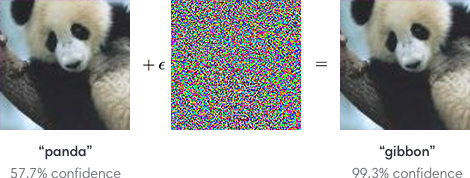
\includegraphics[scale=.75]{attackidea.png}\\
\end{center}
The different algorithms were then coded into R and placed into the given code for the model to be tested and analyzed. The algorithms were tried individually then combined and weighted to be tested together. The rest of the report after detailing the different algorithms shows the testing, correctness, verification, computation complexity with run time and walltime, and overall performance. \\

\addcontentsline{toc}{section}{Adversarial Attacks}
\section*{Adversarial Attacks}
As stated previously, adversarial attacks alter images by adding noise to fool classifiers. They can be problematic in the real world because they affect the validity and usefulness of classifiers. The attacks alter the results decreasing the accuracy and causing incorrect conclusions that can be harmful, especially depending on the initial use of the classifier. It may flag an important email as spam, let a faulty product be sold, or cause a patient to receive proper care. Understanding and being able to recognize and avoid adversarial attacks can help to ensure that classifiers are able to appropriately and accurately do their job. They can be combated by using detectors or separate models rejecting adversarial examples. One can also implement preprocessing, denoising, and principal component analysis. Lastly, to fight adversarial attacks, adversarial training can be used, which is training with adversarial examples, so the model is more prepared. \\
There are white box and black box adversarial attacks both working to fool neural networks into making incorrect conclusions by adding noise, but white box attacks allow for complete access to the architecture, input, and output of the model while black box only allows access to the model input and output. The different attack types employed in this project were found through researching and comparing. In the end, five algorithms were chosen including FGSM, DeepFool, Particle Swarm, CW, and PGD. These use different approaches of adding noise including finding and applying the smallest possible perturbations as well as taking small gradient steps. They were chosen because of the large amount of information already existing on them and their success; however, other potential algorithms are also popular and could have been used include hill climbing or simulated annealing. \\
\noindent{\bf Algorithm 1 - Fast Gradient Sign Method}\\
The fast gradient sign method (FGSM) is a white box attack with a goal of misclassification. It calculates the losses after forward propagation, then calculates the gradient with respect to the image pixels, and finally adjusts the pixels of the images slightly in the direction of the gradients maximizing the loss. The image below shows the potential output of this kind of attack.\\

\begin{center}
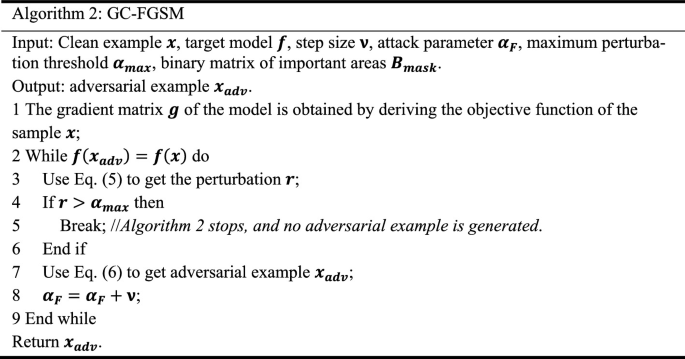
\includegraphics[scale=.45]{FGSMpseudo.png}\\
\caption{Figure 1: The figure above is pseudocode for the FGSM adversarial attack.}\\
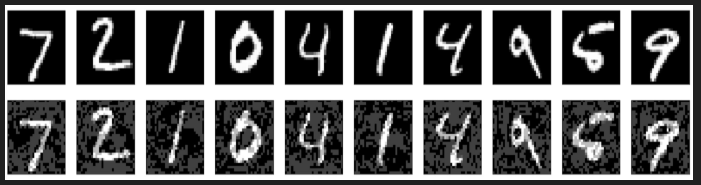
\includegraphics[scale=.75]{FGSM.png}\\
\caption{Figure 2: The image above is an example application of an FGSM attack.}\\
\end{center}

\noindent{\bf Algorithm 2 - DeepFool}\\
This algorithm is a type of white box attack algorithm that adds the minimum necessary perturbations to an image that will lead to a change in the classification label. It can be applied to multiclass or binary classifiers, but for this project, we are focused only on binary classifiers. The pseudocode for the algorithm as well as an example case can be seen below. \\

\begin{center}
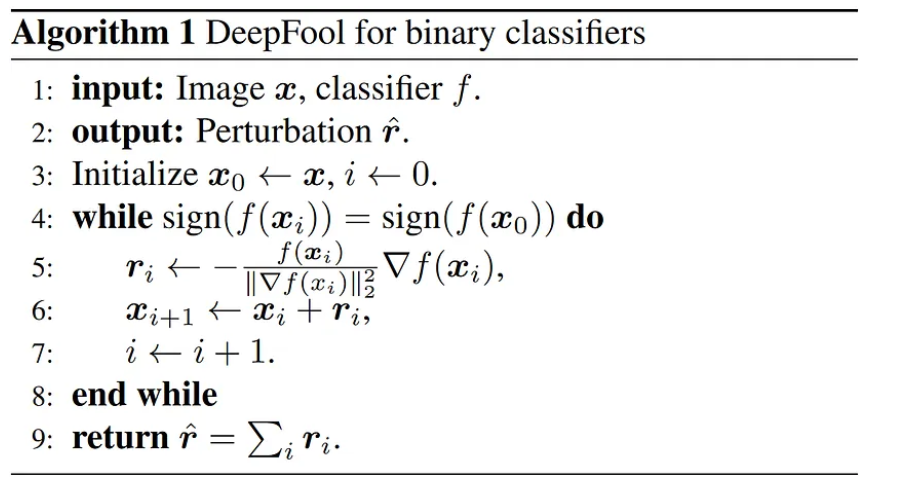
\includegraphics[scale=.5]{deepfoolpseudo.png} \\
\caption{Figure 3: The figure above is pseudocode for the DeepFool adversarial attack.}\\
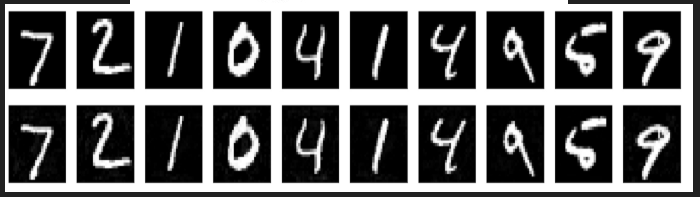
\includegraphics[scale=.75]{deepf.png}\\
\caption{Figure 4: The image above is an example application of a DeepFool attack.}\\
\end{center}

\noindent{\bf Algorithm 3 - Particle Swarm Optimization}\\
This particle swarm optimization (PSO) algorithm operates by finding the local optima and changing them until the classifier can be successfully fooled into incorrectly classifying an image. The pseudocode and possible run for this algorithm is displayed below.\\
\begin{center}
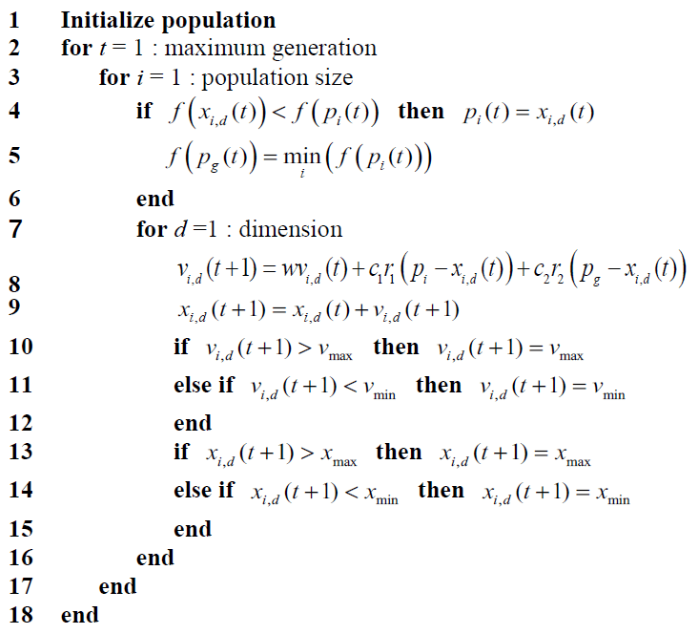
\includegraphics[scale=.5]{particleswarmpseudo.png} \\
\caption{Figure 5: The figure above is pseudocode for the PSO adversarial attack.}\\
\end{center}

\noindent{\bf Algorithm 4 - Carlini Wagner}\\
The Carlini Wagner (CW) algorithm is an iterative attack that calculates and adds perturbations to increase the chance that the image is incorrectly classified. A potential application of the algorithm can be viewed below.\\
\begin{center}
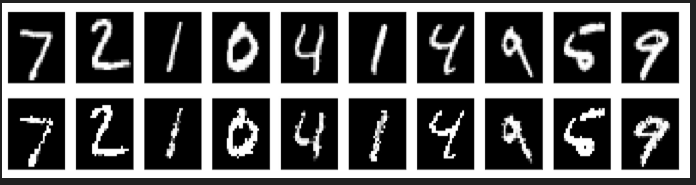
\includegraphics[scale=.75]{CW.png} \\
\caption{Figure 6: The image above is an example application of a CW attacks.}
\end{center}

\noindent{\bf Algorithm 5 - Projected Gradient Descent}\\
Projected gradient descent (PGD) is an algorithm similar to FGSM; however, it calculates a new gradient each iteration with smaller perturbations helping to choose a more ideal stepping size for the attack. An example output is depicted below.\\
\begin{center}
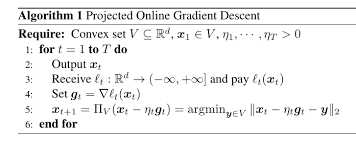
\includegraphics[scale=.65]{PGDpseudo.png} 
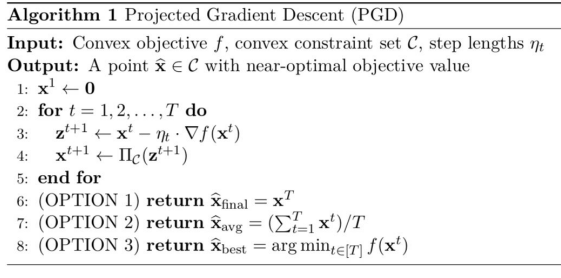
\includegraphics[scale=.54]{PGDpseudo2.png} \\
\caption{Figure 7: The figure above is different pseudocode for the PGD adversarial attack.}\\
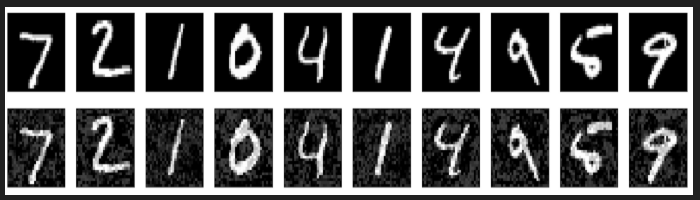
\includegraphics[scale=.75]{PGD.png} \\
\caption{Figure 8: The image above is an example application of a PGD attack.} 
\end{center}

\addcontentsline{toc}{section}{Alternate Approaches}
\section*{Alternate Approaches}
The adversarial attacks were understood and our group worked to implement them; however, despite finding multiple Python codes, no R code was found. We worked to then translate the code we found into R but encountered numerous problems with finding similar packages and functions. As a result, we developed new algorithms that change a larger portion of the image in an attempt to have a working solution that can fool the binary classifier. These were written utilizing different functions made possible from R packages, specifically magick.\\
\noindent{\bf Alternate Algorithm 1 - Grayscale}\\
This converts the colored image into grayscale, which is a black, gray, and white image, which helped to fool the binary classifier since it dulled the image. The image\_colorize function with the "gray" constraint was able to do this. \\
\noindent{\bf Alternate Algorithm 2 - Noise}\\
This approach added noise to the image. Our group used the image\_noise function in R with "gaussian" as the noise type constraint. \\
\noindent{\bf Alternate Algorithm 3 - Coloring}\\
For this method, the images were tinted red, a color that matched neither class. This attempt was made to trick the classifier into incorrectly classifying the images. This was completed using the image\_colorize R function with constraints of color and opacity.\\
\noindent{\bf Alternate Algorithm 4 - Blurring}\\
This approach blurred the image to try and reduce the confidence of the classifier and ultimately fool it. This used the image\_blur R function, which has inputs of the image, radius, and sigma.\\
\noindent{\bf Alternate Algorithm 5 - Embossing}\\
Embossing an image replaces pixels with dark or light colors depending on the surroundings. This was implemented using the image\_emboss function in R, which takes in an image, radius, and sigma.\\

% Testing/Correctness/Verification
\section{Testing/Correctness/Verification}
Each algorithm was tested, analyzed for correctness, and verified to ensure it was properly functioning. Testing was done by running the code and considering the errors encountered as well as the output accuracy. Loop invariants were used to complete the correctness with checking the initialization, maintenance, termination, and correctness. The initialization checks the invariant holds before the loop starts, maintenance ensures the invariant is true throughout the entire iteration, termination focuses on having the algorithm terminate, and correctness finally confirms that the invariant holds when the loop terminates. Lastly, verification, which is different then validation, was ensured by returning to the conceptual model and ensuring the one we developed is representative. Verification looks at whether or not the computational model represents the conceptual while validation considers if the computational model is consistent with the actual system considered. While both are important, we are more concerned with verification in this project. \\
\addcontentsline{toc}{section}{Adversarial Attacks}
\section*{Adversarial Attacks}
\noindent{\bf Algorithm 1 - Fast Gradient Sign Method}\\
The main idea of the Fast Gradient Sign Method (FGSM) is to use the gradient to create perturbation and then add it back to the original image with a certain $\epsilon$. \\
\noindent{\bf Algorithm 2 - DeepFool}\\
For the DeepFool algorithm, the loop invariant statement is the perturbation. The perturbation is initially 0, and there is no noise to be applied to the initial image to create the new image that will later fool the classifier. The while loop then starts under the condition that each part and pixel of the initial image matches the new image. This is checked and if it is true, the perturbation is calculated and applied. It continues to iterate this i number of times with calculating and applying the new perturbation of each part of the image corresponding to i until the entire initial image has been processed and new image developed. The loop will then terminate and returns the sum of i perturbations with a new image that has the perturbations applied causing it to fool the classifier.\\
\noindent{\bf Algorithm 3 - Particle Swarm Optimization}\\
The loop invariant for PSO there are multiple loops. For the first loop the invariant is that the minimum is located and stored. It starts with an initialized function of values, checks if the next function has values smaller, and if so it sets that minimum value of that function as the comparator. This loop is continued through the entire population then terminates ensuring that all of the local minimum are found and recorded. The next loop is focused on applying the noise to alter the image at the local minimum. The loop invariant is the image alteration. The loop starts with the initial image and goes through the entire dimensions appropriately applying values to the different image parts and pixels based on the different conditions. This continues until it terminates once the entire image is altered as needed.\\
\noindent{\bf Algorithm 4 - Carlini Wagner}\\
\noindent{\bf Algorithm 5 - Projected Gradient Descent}\\

\addcontentsline{toc}{section}{Alternate Approaches}
\section*{Alternate Approaches}
Each of these used built-in functions from the R package magick, so there is no loop for us to find the invariant and check correctness. Testing was able to be completed by running each function and analyzing the outputs. Verification was done by ensuring it matched the goals set. 
\noindent{\bf Alternate Algorithm 1 - Grayscale}\\
This successfully applied gray to the image dulling it, which was the goal. It does affect the entire image rather than 10 percent and helps to fool the image classifier on certain cases.
\noindent{\bf Alternate Algorithm 2 - Noise}\\
Noise is correctly added to each image and the amount can be set to match the 10 percent constraint provided. While it has helped to fool the classifier in many cases, it doesn't have 100 percent accuracy in fooling it. \\
\noindent{\bf Alternate Algorithm 3 - Coloring}\\
The image receives a red tint when this function is applied like intended. This again affects the whole image rather than 10 percent but yielded a good proportion of fooling with the images.\\
\noindent{\bf Alternate Algorithm 4 - Blurring}\\
Blurring is applied to the entire image appropriately; however, this doesn't match the entirety of the project's constraints. \\
\noindent{\bf Alternate Algorithm 5 - Embossing}\\
Each image is embossed when this function is run on it. This could be set to 10 percent of the image; however, doesn't fool the classifier in every case like hoped. \\
\section{Runtime Complexity and Walltime}
Runtime complexity analyzes the computational complexity of an algorithm to develop an idea of how long it will take to run based on a function for the input size n. For this, the input n would be the number of iterations determined by the number of pixels the algorithm must change before the classifier is finally fooled. The functions can include using Big-Oh, Big-Omega, and Big-Theta as models. Big-Oh focuses on creating an upper bound function, Big-Omega focuses on creating a lower bound function, and lastly Big-Theta makes a tight bound with one function being implemented as a lower and upper bound depending on the constant. Walltime is the actual numerical time the algorithm took when running calculated by a clock.
\\
A lower runtime and walltime is preferred because it is not convenient nor efficient to have to wait long periods of time for an output; however, there is usually a tradeoff in complexity and runtime, especially when considering the number of iterations. This tradeoff is important to consider when developing and implementing different algorithms. The amount of time can also depend on the technology one is using, so investing in better, more advanced technology may be helpful in reducing the wait time and allow for more complex algorithms to take less time.\\
\addcontentsline{toc}{section}{Adversarial Attacks}
\section*{Adversarial Attacks}
Unfortunately, since we were unable to get adversarial attacks working, we were also not able to evaluate their walltime. We were able to look a little into the runtime based on the pseudocode and python code. If we were able to better determine these factors, we would have found the different T(n) functions and bounds for the runtime and recorded the time the code took for walltime. From here, we could have compared this to see which took the longest.
\addcontentsline{toc}{section}{Alternate Approaches}
\section*{Alternate Approaches}
\noindent{\bf Alternate Algorithm 1 - Grayscale}\\

\noindent{\bf Alternate Algorithm 2 - Noise}\\

\noindent{\bf Alternate Algorithm 3 - Coloring}\\

\noindent{\bf Alternate Algorithm 4 - Blurring}\\

\noindent{\bf Alternate Algorithm 5 - Embossing}\\


\section{Performance}
The overall performance of the algorithms was analyzed using the outputs, runtime, and walltime to see how well they worked and their overall efficiency. It combines both the testing/correctness/verifcation and runtime complexity and walltime. Performance is important in determining which methods to implement and develop the weighted algorithm.\\
There tends to be tradeoffs with performance, which we addressed briefly in the last section. Increasing complexity may help to improve correctness; however, it may take longer time to run. Performance of algorithms also depend on other factors. Again, the technology used plays a part in efficiency. The models that are analyzed can also determine performance, as training data size can affect fitting, which may help or hinder performance. Using too much training data may cause overfitting, as it becomes too specific to that data. On the other end, using too little data can lead to underfitting because the model can't gather enough information to make strong predictions. It is important to understand these concepts when developing models and algorithms to ensure they perform well. \\
\addcontentsline{toc}{section}{Adversarial Attacks}
\section*{Adversarial Attacks}
Unfortunately, since we were unable to get adversarial attacks working, we were also not able to evaluate their performance. We would assume these attacks would work well in fooling the classifier if they had been fully developed because of the extensive information and feedback on them from others. There are also videos and papers online showing them implemented and working, so we know that the logic works and can be applied to successfully fool classifiers. \\
\addcontentsline{toc}{section}{Alternate Approaches}
\section*{Alternate Approaches}
\noindent{\bf Alternate Algorithm 1 - Grayscale}\\

\noindent{\bf Alternate Algorithm 2 - Noise}\\

\noindent{\bf Alternate Algorithm 3 - Coloring}\\

\noindent{\bf Alternate Algorithm 4 - Blurring}\\
\noindent{\bf Alternate Algorithm 5 - Embossing}\\

\pagebreak
\newquestion{References}
\section{References}

%APPENDIX
\pagebreak
\newquestion{Appendices}
\section{Appendix}
\addcontentsline{toc}{section}{Challenges}
\section*{Challenges}
The main challenges faced were successfully implementing the found adversarial attacks. After our research, we worked to develop these into working codes to later be applied to images; however, due to lack of knowledge and experience in R and limited time, we couldn't complete this. We continued to familiarize ourselves with these algorithms and share them to be used in the future and instead tried new approaches that are more drastic. These included changing color and resolution of the images to fool the classifier. With these algorithms, it was difficult to adhere to only changing 10 percent of pixels. As a result, we worked to limit their affects on the overall image as a compromise. \\
In the end, we put our focus on the report with showing our knowledge, process, and work. We gave background and guidance on implementing the traditional adversarial attacks as well as included the information and code for the alternate algorithms in R that we were able to apply. \\
\addcontentsline{toc}{section}{Algorithms}
\section*{Algorithms}

\begin{lstlisting}[language=R, frame=single]
#FGSM Algorithm
FGSM <- function(type, file_name, epsilon){
  
  #load model
  model2 <- keras::application_mobilenet_v2(weights = "imagenet")
  knitr::knit_engines$set(python = reticulate::eng_python) 
  
  # Preprocess input data
  x <- image_load(paste("./test_photos/",type,"/",file_name,".jpg",sep = ""), target_size = c(224, 224))
  x <- image_to_array(x)
  x <- array_reshape(x, c(1, dim(x)))
  x <- tf$convert_to_tensor(x, dtype = "float32") #change x to tensor
  
  # Predict first using the model
  pred <- model2(x)
  pred_shape <- tf$shape(pred)
  pred <- tf$cast(pred, "float32")
  
  #label
  labrador_retriever_index <- 208
  label <- k_one_hot(as.integer(labrador_retriever_index), tf$shape(pred)[-1])
  label <- tf$reshape(label, shape = c(as.integer(1), tf$shape(pred)[-1]))
  
  #get the gradient
  with(tf$GradientTape() %as% tape, {
    tape$watch(x)
    pred <- model2(x)
    loss <- k_categorical_crossentropy(label, pred)
    grads <- tape$gradient(loss,x)
  })
  
  #get the sign of gradient
  signed <- tf$sign(grads)
  
  #let's get the perturbations
  perturbations <- signed
  
  #set the epsilons and add the perturbations
  epsilon <- epsilon
  adv_x <- x + epsilon * perturbations
  
  #plot image
  adv_x_matrix <- matrix(adv_x, nrow=dim(adv_x)[1]*dim(adv_x)[2], ncol=dim(adv_x)[3])
  adv_x_2d <- (adv_x_matrix * 0.5) + 0.5
  par(mar=c(1,1,1,1))
  a <- image(adv_x_2d)

}
\end{lstlisting}
\begin{lstlisting}[language=Python, frame=single]
#DeepFool Algorithm
import numpy as np
from torch.autograd import Variable
import torch as torch
import copy
from torch.autograd.gradcheck import zero_gradients


def deepfool(image, net, num_classes=10, overshoot=0.02, max_iter=50):
  
  """
       :param image: Image of size HxWx3
       :param net: network (input: images, output: values of activation **BEFORE** softmax).
       :param num_classes: num_classes (limits the number of classes to test against, by default = 10)
       :param overshoot: used as a termination criterion to prevent vanishing updates (default = 0.02).
       :param max_iter: maximum number of iterations for deepfool (default = 50)
       :return: minimal perturbation that fools the classifier, number of iterations that it required, new estimated_label and perturbed image
    """
is_cuda = torch.cuda.is_available()

if is_cuda:
  print("Using GPU")
image = image.cuda()
net = net.cuda()
else:
  print("Using CPU")


f_image = net.forward(Variable(image[None, :, :, :], requires_grad=True)).data.cpu().numpy().flatten()
I = (np.array(f_image)).flatten().argsort()[::-1]

I = I[0:num_classes]
label = I[0]

input_shape = image.cpu().numpy().shape
pert_image = copy.deepcopy(image)
w = np.zeros(input_shape)
r_tot = np.zeros(input_shape)

loop_i = 0

x = Variable(pert_image[None, :], requires_grad=True)
fs = net.forward(x)
fs_list = [fs[0,I[k]] for k in range(num_classes)]
k_i = label

while k_i == label and loop_i < max_iter:
  
  pert = np.inf
fs[0, I[0]].backward(retain_graph=True)
grad_orig = x.grad.data.cpu().numpy().copy()

for k in range(1, num_classes):
  zero_gradients(x)

fs[0, I[k]].backward(retain_graph=True)
cur_grad = x.grad.data.cpu().numpy().copy()

# set new w_k and new f_k
w_k = cur_grad - grad_orig
f_k = (fs[0, I[k]] - fs[0, I[0]]).data.cpu().numpy()

pert_k = abs(f_k)/np.linalg.norm(w_k.flatten())

# determine which w_k to use
if pert_k < pert:
  pert = pert_k
w = w_k

# compute r_i and r_tot
# Added 1e-4 for numerical stability
r_i =  (pert+1e-4) * w / np.linalg.norm(w)
r_tot = np.float32(r_tot + r_i)

if is_cuda:
  pert_image = image + (1+overshoot)*torch.from_numpy(r_tot).cuda()
else:
  pert_image = image + (1+overshoot)*torch.from_numpy(r_tot)

x = Variable(pert_image, requires_grad=True)
fs = net.forward(x)
k_i = np.argmax(fs.data.cpu().numpy().flatten())

loop_i += 1

r_tot = (1+overshoot)*r_tot

return r_tot, loop_i, label, k_i, pert_image
\end{lstlisting}
\begin{lstlisting}[language=R, frame=single]
#PSO Algorithm
tictoc::tic()
psoptim(par = rep(NA,2), fn = fit_function, lower = c(1,1), upper = c(17, 128), 
        control = list(maxit = 1000, maxit.stagnate = 10, vectorize = T, s = 100))
\end{lstlisting}
\begin{lstlisting}[language=Python, frame=single]
#CW Algorithm
from keras.models import Sequential
from keras.layers import Input, Lambda,  Flatten

batch_size = 1
 
m = Sequential()

# newInput expect an image ranging [-0.5,0.5] --> need to transform to our range: [0,1] by multipying all the values by 2
m.add(Lambda(lambda x : x+0.5,name="rescaledm05p05",input_shape=(28,28,1)))

## start from 1 because we want to use new Input layer 
## end right before -1 because softmax should be removed. 
for l in model_keras.layers[:-1]:
    #print(l.name)
    m.add(l)
#m.add(Flatten())
# https://github.com/keras-team/keras/issues/8909
model_rescaled = m
model_rescaled.summary()
from nn_robust_attacks.l0_attack import CarliniL0
# model must be tensorflow model model_tf = KerasModelWrapper(model.model)


class ModelWrapper:
    def __init__(self,keras_model,num_labels=10):
        self.model = keras_model
        self.num_channels = self.model.input_shape[-1]
        self.image_size = self.model.input_shape[1] ## assume height = width
        self.num_labels = num_labels
    def predict(self, data):
        return self.model(data)        

num_classes = 10   
model_attack = ModelWrapper(model_rescaled,num_classes) 
attack = CarliniL0(sess,model_attack,
                   ## learning rate needed to be reduced from default for mobilenet
                   learning_rate = 0.01,
                   targeted=True,
                   max_iterations=10000, 
                   initial_const=10,
                   largest_const=15)
\end{lstlisting}
\begin{lstlisting}[language=Python, frame=single]
#PGD Algorithm
import torch

def projected_gradient_descent(model, x, y, loss_fn, num_steps, step_size, step_norm, eps, eps_norm,
                               clamp=(0,1), y_target=None):
  """Performs the projected gradient descent attack on a batch of images."""
x_adv = x.clone().detach().requires_grad_(True).to(x.device)
targeted = y_target is not None
num_channels = x.shape[1]

for i in range(num_steps):
  _x_adv = x_adv.clone().detach().requires_grad_(True)

prediction = model(_x_adv)
loss = loss_fn(prediction, y_target if targeted else y)
loss.backward()

with torch.no_grad():
  # Force the gradient step to be a fixed size in a certain norm
  if step_norm == 'inf':
  gradients = _x_adv.grad.sign() * step_size
else:
  # Note .view() assumes batched image data as 4D tensor
  gradients = _x_adv.grad * step_size / _x_adv.grad.view(_x_adv.shape[0], -1)\
.norm(step_norm, dim=-1)\
.view(-1, num_channels, 1, 1)

if targeted:
  # Targeted: Gradient descent with on the loss of the (incorrect) target label
  # w.r.t. the image data
  x_adv -= gradients
else:
  # Untargeted: Gradient ascent on the loss of the correct label w.r.t.
  # the model parameters
  x_adv += gradients

# Project back into l_norm ball and correct range
if eps_norm == 'inf':
  # Workaround as PyTorch doesn't have elementwise clip
  x_adv = torch.max(torch.min(x_adv, x + eps), x - eps)
else:
  delta = x_adv - x

# Assume x and x_adv are batched tensors where the first dimension is
# a batch dimension
mask = delta.view(delta.shape[0], -1).norm(norm, dim=1) <= eps

scaling_factor = delta.view(delta.shape[0], -1).norm(norm, dim=1)
scaling_factor[mask] = eps

# .view() assumes batched images as a 4D Tensor
delta *= eps / scaling_factor.view(-1, 1, 1, 1)

x_adv = x + delta

x_adv = x_adv.clamp(*clamp)

return x_adv.detach()
\end{lstlisting}
\begin{lstlisting}[language = R, frame=single]
#Alternate Algorithm
# Load packages
library(tidyverse)
library(keras)
library(tensorflow)
library(reticulate)
library(R6)

setwd(dirname(rstudioapi::getActiveDocumentContext()$path))

# Image class
Image <- R6Class("Image",
    public = list(
        type = NULL,
        file_name = NULL,
        original_path = NULL,
        test_path = NULL,
        img = NULL,

        # constructor
        initialize = function(type, file_name) {
            self$type <- type
            self$file_name <- file_name
            self$original_path <- paste("./original_photos/", type, "/", file_name, sep = "")
            self$test_path <- paste("./test_photos/", type, "/", file_name, sep = "")
        },

        # open test image
        open_test = function() {
            system(paste("open 'test_photos/", self$type, "/", self$file_name, "'", sep = ""))
        },
        open_original = function() {
            system(paste("open 'original_photos/", self$type, "/", self$file_name, "'", sep = ""))
        },

        # function to check if an image is a dandelion or grass
        check = function() {
            test_image <- image_load(self$test_path, target_size = c(224, 224))
            x <- image_to_array(test_image)
            x <- array_reshape(x, c(1, dim(x)))
            x <- x / 255
            pred <- model %>% predict(x)

            print(paste("File Name:", self$file_name))
            print(paste("Actual Type:", self$type))
            if (pred[1, 1] < 0.50) {
                print("Predicted Type: 'grass'")
                print("With Confidence:")
                print(pred[1, 2])
            } else if (pred[1, 2] < 0.50) {
                print("Predicted Type: dandelions")
                print("With Confidence:")
                print(pred[1, 1])
            } else {
                print("ERROR")
            }
        }
    )
)

# initialize model
model <- load_model_tf("./dandelion_model")

# initialize vector of all test images
all_images <- c()
for (type in c("grass", "dandelions")) {
    for (file in list.files(paste("./test_photos/", type, sep = ""))) {
        all_images <- append(all_images, Image$new(type, file))
    }
}

# function to reset test images
reset_test_images <- function() {
    source_folder <- "./original_photos"
    destination_folder <- "./test_photos"

    # Create destination folder if it doesn't exist
    if (!dir.exists(destination_folder)) {
        dir.create(destination_folder)
    }

    # Copy files from source to destination
    for (f in list.files(source_folder)) {
        file.copy(from = file.path(source_folder, f), to = destination_folder, overwrite = TRUE, recursive = TRUE)
    }
}

# function to check test images
check_test_images <- function() {
    for (image in all_images) {
        image$check()
    }
}

# script
reset_test_images()

# algorithm
library(magick)

launch_attack <- function(weights = c(0.2, 0.2, 0.2, 0.2, 0.2)) {
    for (image in all_images) {
        img <- image_read(image$original_path)

        # add color filter
        img <- image_colorize(img, weights[1] * 50, "red")

        # add grayscale filter
        img <- image_colorize(img, weights[2] * 50, "gray")

        # add noise
        img <- image_noise(img, "gaussian")

        # add blur
        img <- image_blur(img, 25, 2)

        # add emboss
        img <- image_emboss(img, 25, 2)

        # save image
        image_write(img, image$test_path)
        print(paste("Modified Image:", image$file_name))
    }
}

launch_attack()

# check results
check_test_images()
    
\end{lstlisting}
\end{document}

#Deepfool
https://neptune.ai/blog/adversarial-attacks-on-neural-networks-exploring-the-fast-gradient-sign-method \\
https://link.springer.com/chapter/10.1007/978-3-031-20500-2_1\\
https://towardsdatascience.com/deepfool-a-simple-and-accurate-method-to-fool-deep-neural-networks-17e0d0910ac0
https://medium.com/machine-intelligence-and-deep-learning-lab/a-review-of-deepfool-a-simple-and-accurate-method-to-fool-deep-neural-networks-b016fba9e48e
https://www.crcv.ucf.edu/wp-content/uploads/2018/11/Lecture-3-DeepFool.pdf
https://ebezzam.github.io/pdf/lts4_semester_project_eric_bezzam.pdf\\

#PGD
https://www.skillsire.com/read-blog/359_a-overview-on-adversarial-attacks-and-defenses.html
file:///C:/Users/ccook/Downloads/Lec-Models-from-Data_Part%20I_%20Projections%20-PGraDescent%202.pdf
https://www.google.com/search?q=pseudocode+for+pgd+algorithm&rlz=1C1UEAD_enUS1046US1046&sxsrf=APwXEdeZYouL7qb_KdHxZA3MeNsuFciXbw:1682641181340&source=lnms&tbm=isch&sa=X&ved=2ahUKEwiasJfvpsv-AhXbkokEHfOmCnoQ0pQJegQIBBAC&biw=1536&bih=746&dpr=1.25#imgrc=OIXv_z01BE3vAM&imgdii=g321OUOe9UuBkM \\

#Particle Swarm
https://www.researchgate.net/figure/Pseudocode-of-standard-particle-swarm-optimization_fig1_323281605
https://rpubs.com/argaadya/intro-pso
https://www.analyticsvidhya.com/blog/2021/10/an-introduction-to-particle-swarm-optimization-algorithm/\\

#CW
https://www.skillsire.com/read-blog/359_a-overview-on-adversarial-attacks-and-defenses.html
https://fairyonice.github.io/Learn-the-Carlini-and-Wagners-adversarial-attack-MNIST.html

#Run Time
https://viso.ai/deep-learning/adversarial-machine-learning/
https://deepchecks.com/glossary/binary-classification/ - info 